\part{Perspectives d'améliorations}
\label{part:ameliorations}

\section{Détection de tag}

    \subsection{Robustesse de la détection}

    Une des faiblesses de notre système de détection de tag est l'impossibilité du système à détecter le tag lorsque ce dernier n'est pas entièrement dans l'écran.

    Implémenter une méthode permettant justement de réussir à estimer la position du tag à partir d'un fragment visible de ce dernier aurait pu s'avérer intéressant, les mouvements de l'utilisateur pouvant faire sortir régulièrement le tag du champ de la caméra.

\section{Techniques de rendu}

    \subsection{Détection des sources lumineuses}

    La lumière dans ce système de réalité augmenté est gérée statiquement : le vecteur représentant la direction de la lumière est invariant selon l'image.
    Détecter les sources lumineuses sur l'image pour modifier image par image la direction de la lumière aurait pu être une manière intéressante d'augmenter le réalisme de l'application, bien que cette détection de source de lumière sur l'image se serait avérée être une tâche probablement nécessitant du temps.

    \subsection{Ombrage de Gouraud}

    Nous avons tenté d'implémenter, sans succès, un ombrage de Gouraud pour le rendu des objets. Cela aurait pu s'avérer intéressant pour un souci de réalisme, l'ombrage de Gouraud interpolant chaque pixel de chaque face pour lui assigner une luminosité différente.

    Malheureusement, OpenCV n'est pas l'outil le plus adapté à ce genre de tâche, ces calculs étaient particulièrement longs à être effectués. Pour parvenir plus facilement à un résultat, nous aurions pu utiliser un moteur de rendu tels qu'OpenGL, ou paralléliser le calcul.

    \begin{figure}[!h]
        \centering
        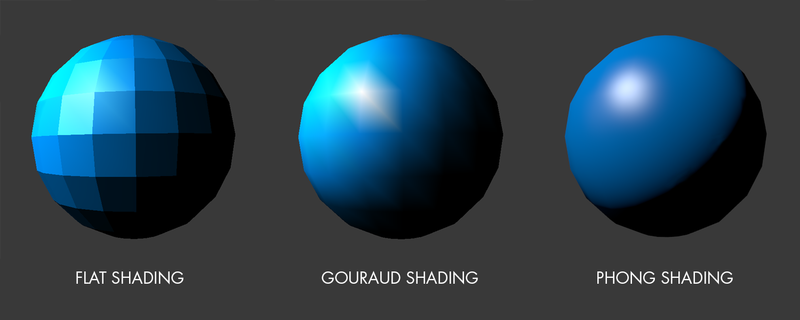
\includegraphics[scale=0.25]{img/shading.png}
        \caption{L'interpolation utilisée dans l'ombrage de Gouraud et de Phong lisse la surface de l'objet et améliore le réalisme du rendu}
    \end{figure}

    \subsection{Performance}

    Nous utilisons OpenCV, bibliothèque de traitement d'image pour le rendu, et non un moteur de rendu spécialisé. Nous avons donc été limités dans certains choix pour cause de performance. L'ombrage plat et la couleur unique pour les faces sont les exemples les plus importants.